% EPR generation time and the compiler-driven (Dynamic) strategy: a measured study.
% Compile with:  tectonic main.tex   (twice, for the table of contents and references).
% Every table in generated/ and every number in generated/numbers.tex is written by
% tools/generation_time_study/make_tables.py from the data in docs/research/generation-time-2026-11-01/data/.
% Every figure in figures/ is written by tools/generation_time_study/figures.py. Nothing is typed in by hand.
\documentclass[11pt,a4paper]{report}
\usepackage[margin=24mm]{geometry}
\usepackage[T1]{fontenc}
\usepackage{url,lmodern,booktabs,longtable,array,amsmath,amssymb,xcolor,graphicx,float,caption,subcaption,hyperref,enumitem,tikz}
\hypersetup{colorlinks=true,urlcolor=blue,linkcolor=black,citecolor=black}
\captionsetup{font=small,labelfont=bf}
\setlength{\parindent}{0pt}\setlength{\parskip}{5pt}\setlength{\emergencystretch}{3em}
\setlist{itemsep=2pt,topsep=2pt}
\graphicspath{{figures/}}
\newcommand{\BaseAttempts}{2.44}
\newcommand{\BaseGenForward}{0.972}
\newcommand{\BaseGenMean}{1.10}
\newcommand{\BaseGenReverse}{1.220}
\newcommand{\BasePSuccess}{0.407}
\newcommand{\BaseQaoaFourComm}{22.7}
\newcommand{\BaseQaoaFourDyn}{0.981}
\newcommand{\BaseQaoaFourGain}{28.0}
\newcommand{\BaseQaoaFourHit}{53.7}
\newcommand{\BaseQaoaFourMakespan}{11.4}
\newcommand{\BaseQaoaFourOdg}{1.364}
\newcommand{\BaseQaoaFourSaving}{0.38}
\newcommand{\BaseQaoaThreeComm}{9.7}
\newcommand{\BaseQaoaThreeDyn}{1.265}
\newcommand{\BaseQaoaThreeGain}{13.0}
\newcommand{\BaseQaoaThreeHit}{38.1}
\newcommand{\BaseQaoaThreeMakespan}{4.9}
\newcommand{\BaseQaoaThreeOdg}{1.454}
\newcommand{\BaseQaoaThreeSaving}{0.19}
\newcommand{\BaseQftFourComm}{43.6}
\newcommand{\BaseQftFourDyn}{0.703}
\newcommand{\BaseQftFourGain}{46.8}
\newcommand{\BaseQftFourHit}{73.6}
\newcommand{\BaseQftFourMakespan}{13.0}
\newcommand{\BaseQftFourOdg}{1.322}
\newcommand{\BaseQftFourSaving}{0.62}
\newcommand{\BaseQftThreeComm}{29.2}
\newcommand{\BaseQftThreeDyn}{0.933}
\newcommand{\BaseQftThreeGain}{31.3}
\newcommand{\BaseQftThreeHit}{55.2}
\newcommand{\BaseQftThreeMakespan}{8.8}
\newcommand{\BaseQftThreeOdg}{1.357}
\newcommand{\BaseQftThreeSaving}{0.42}
\newcommand{\BreakEvenCases}{188}
\newcommand{\BreakEvenLosing}{40}
\newcommand{\BreakEvenLosingBreak}{41}
\newcommand{\BreakEvenLosingHit}{20}
\newcommand{\CasesAccepted}{548}
\newcommand{\FunnelAcceptedZero}{35.9}
\newcommand{\FunnelExpiredZero}{6.3}
\newcommand{\FunnelHitFive}{73.6}
\newcommand{\FunnelHitZero}{19.7}
\newcommand{\FunnelMissWaitFive}{0.10}
\newcommand{\FunnelMissWaitZero}{0.59}
\newcommand{\FunnelOdgWait}{0.008}
\newcommand{\FunnelPrep}{1.11}
\newcommand{\FunnelRejectZero}{80}
\newcommand{\FunnelSlackFive}{9.9}
\newcommand{\FunnelSlackZero}{1.4}
\newcommand{\LinkPairs}{360\,200}
\newcommand{\LinkProbes}{110}
\newcommand{\LowQaoaFourGain}{22.3}
\newcommand{\LowQaoaFourGen}{10.5}
\newcommand{\LowQaoaFourSaving}{2.57}
\newcommand{\LowQaoaThreeGain}{6.5}
\newcommand{\LowQaoaThreeGen}{10.5}
\newcommand{\LowQaoaThreeSaving}{0.80}
\newcommand{\LowQftFourGain}{51.2}
\newcommand{\LowQftFourGen}{10.6}
\newcommand{\LowQftFourSaving}{5.85}
\newcommand{\LowQftThreeGain}{31.8}
\newcommand{\LowQftThreeGen}{10.6}
\newcommand{\LowQftThreeSaving}{3.72}
\newcommand{\MemQftEight}{65}
\newcommand{\MemQftTwo}{3}
\newcommand{\PeakQaoaFourEff}{0.6}
\newcommand{\PeakQaoaFourGain}{36.8}
\newcommand{\PeakQaoaFourGen}{2.8}
\newcommand{\PeakQaoaThreeEff}{0.6}
\newcommand{\PeakQaoaThreeGain}{19.3}
\newcommand{\PeakQaoaThreeGen}{2.8}
\newcommand{\PeakQftFourEff}{0.6}
\newcommand{\PeakQftFourGain}{59.4}
\newcommand{\PeakQftFourGen}{2.8}
\newcommand{\PeakQftThreeEff}{0.6}
\newcommand{\PeakQftThreeGain}{41.4}
\newcommand{\PeakQftThreeGen}{2.8}
\newcommand{\PredAttempts}{2.46}
\newcommand{\QftGapFiveBreak}{8.7}
\newcommand{\QftGapFiveRest}{1.41}
\newcommand{\QftGapZeroBreak}{40.4}
\newcommand{\QftGapZeroGain}{$-$19.5}
\newcommand{\QftGapZeroHit}{19.7}
\newcommand{\QftGapZeroRest}{1.83}
\newcommand{\QftHitCost}{0.45}
\newcommand{\QftOdgMs}{1.32}
\newcommand{\ReadyQaoaError}{3.7}
\newcommand{\ReadyQftError}{0.7}
\newcommand{\ReadyTrials}{656}
\newcommand{\RetryQaoaDefault}{$-$59}
\newcommand{\RetryQaoaScaled}{24}
\newcommand{\TotalTrials}{4\,144}
\newcommand{\TuningCases}{110}
\newcommand{\ValidationHold}{8}
\newcommand{\ValidationTotal}{8}

\newcommand{\code}[1]{\texttt{\detokenize{#1}}}
\newcommand{\ms}{\,ms}
\newcommand{\us}{\,\ensuremath{\mu\mathrm{s}}}
\newcommand{\fit}[1]{\resizebox{\linewidth}{!}{\input{#1}}}
\newcommand{\gain}{\mathrm{gain}}
\newenvironment{plain}{\begin{quote}\small\itshape}{\end{quote}}
\definecolor{note}{HTML}{f1f0ec}
\newcommand{\finding}[1]{\par\medskip\noindent\colorbox{note}{\parbox{\dimexpr\linewidth-2\fboxsep}{\textbf{Finding.} #1}}\par\medskip}
\title{When does it pay to prepare EPR pairs in advance?\\[3pt]\large A measured study of EPR generation time\\and the compiler-driven Dynamic strategy}
\author{BTP, MARS Lab, IIT Guwahati}
\date{2 November 2026}

\begin{document}
\maketitle
\begin{abstract}\noindent
The ACE simulator delivers an EPR pair between two neighbouring cores either \emph{on demand} (ODG), when a request needs it, or in advance, when the compiler has planned it (\emph{Dynamic}). The idea behind this study is that a slower pair generation hurts ODG more, so Dynamic should look better. We measured that idea directly: the generation time of a single pair on the real simulator (\LinkPairs{} pairs), then \TotalTrials{} full-workload trials across \CasesAccepted{} audited cases (shared base cases counted once) that vary the physical parameters, the time constants hidden in the simulator, and Dynamic's own options.
Generation time is $(4\text{ or }5)\,\delta/p$: about \BaseGenMean{}\ms{} for one pair at the baseline. Slower generation does help Dynamic, but only up to a point, and only because of a time constant that is not physical: the 5\ms{} charged for every layer without inter-core requests. Without it, default Dynamic is \emph{worse} than ODG at normal speed. We explain why with a break-even model and a funnel of what happens to every planned pair, show that the best Dynamic options validate on unseen seeds, and list what to change in the simulator and what to ask the supervisor.
\end{abstract}
\tableofcontents

\chapter{The question and the short answers}
\section{The idea}
Creating an EPR pair between two cores is probabilistic: it can fail and must be retried, and each try needs several classical messages. ODG pays this time \emph{inside} the request. Dynamic uses the circuit's known future requests to start the pair earlier, in a quiet moment, so that the request finds it ready. The idea we tested is simple: \emph{the longer a pair takes to make, the more ODG suffers and the more Dynamic gains.}

\section{Short answers}
\begin{enumerate}
\item \textbf{What is the generation time?} For one hop, $T_{\text{gen}} = (4\text{ or }5)\,\delta\,/\,p$, where $\delta$ is the classical message delay ($100\us{}$ by default), $p=\BasePSuccess{}$ is the success chance of one attempt, and the factor is 4 for a hop whose source core has the lower number and 5 for the reverse hop. The mean is \BaseGenMean{}\ms{} (\BaseGenForward{}\ms{} forward, \BaseGenReverse{}\ms{} reverse) after $\BaseAttempts{}$ attempts on average. This was measured on \LinkPairs{} pairs and matched the formula in every probe for the number of attempts (Chapter~\ref{ch:anatomy}).
\item \textbf{Which knobs change it?} The classical delay, and anything that changes $p$: memory efficiency, detector efficiency, the BSM success rate, and link loss. Memory excitation rate matters only below about 5\,kHz (the default is 80\,MHz). Coherence time, fidelity settings, gate settings and the empty-layer gap do not change it (Chapter~\ref{ch:knobs}).
\item \textbf{Does slower generation help Dynamic?} Yes at first. On QFT with $M=4$ the latency gain over ODG rises from \BaseQftFourGain{}\% at the baseline to a peak of \PeakQftFourGain{}\% when ODG generation takes \PeakQftFourGen{}\ms{}, then falls to \LowQftFourGain{}\% at \LowQftFourGen{}\ms{}, because pairs no longer finish before they are needed. The \emph{absolute} saving keeps growing, from \BaseQftFourSaving{}\ms{} to \LowQftFourSaving{}\ms{} per hop (Chapter~\ref{ch:sweeps}).
\item \textbf{What is the catch?} The gain depends on a 5\ms{} constant that gives every empty layer five milliseconds. With it, preparations finish in the quiet time (\FunnelSlackFive{}\ms{} between launch and request, against \FunnelPrep{}\ms{} to make a pair). With no gap, only \FunnelHitZero{}\% of requests find a ready pair, memory contention pushes the others \FunnelMissWaitZero{}\ms{} later, and Dynamic is \QftGapZeroGain{}\% against ODG on QFT (Chapter~\ref{ch:gap}).
\item \textbf{Can Dynamic be improved?} Yes, and the improvement holds on unseen seeds. Letting Dynamic use all memories (C=M) cuts QFT latency by 16--24\%, and borrowing pairs or demand-first cuts QAOA latency by 7--14\%. Many popular options hurt, and a longer lead hurts badly (Chapter~\ref{ch:tuning}).
\item \textbf{What should we be careful about?} Absolute latencies rest on two assumed constants ($\delta=100\us{}$, taken from a metro-scale paper, and the 5\ms{} gap). Every claim here is a ratio, a regime, or a mechanism, and the report says which (Chapter~\ref{ch:limits}).
\end{enumerate}

\section{How to read the numbers}
\begin{itemize}
\item \textbf{Latency} is the mean time per hop from when a request becomes eligible until its EPR pair is delivered. Data teleportation and local gates are not simulated.
\item \textbf{Gain} is $100\times(1-\text{Dynamic}/\text{ODG})$ on the same route, memories, seeds and settings. A negative gain means Dynamic is worse.
\item \textbf{Hit} means the pair was ready before the request was first submitted.
\item \textbf{Makespan} is the time to finish the whole workload. \textbf{Communication time} is the makespan minus the empty-layer gaps.
\item Intervals are 95\% Student-$t$ intervals over seeds. Seeds change the simulator's random numbers, not the circuit or its mapping.
\end{itemize}

\chapter{System and baseline}
\section{How a pair is made}
A hop moves a qubit between two neighbouring cores on a $4\times4$ mesh. The pair is made between one memory in each core, with a Bell-state measurement station (BSM) halfway between them. One \emph{attempt} runs four steps: a pairing handshake, a NEGOTIATE message that agrees when both cores emit, both cores emit a photon towards the BSM, and a heralding message back from the BSM that says whether it worked. The photons themselves fly in about 125\,ps. Every other step is a classical message that takes $\delta$. An attempt succeeds with probability
\[ p \;=\; r_{\text{BSM}}\,\bigl(\eta_{\text{mem}}\,\eta_{\text{det}}\,\eta_{\text{fibre}}\bigr)^{2},\qquad r_{\text{BSM}}=0.5,\ \eta_{\text{mem}}=\eta_{\text{det}}=0.95,\ \eta_{\text{fibre}}\approx1, \]
so $p=\BasePSuccess{}$ at the baseline. The expression comes from the engine's BSM code and is checked in Chapter~\ref{ch:knobs}.

\section{The two strategies}
\textbf{ODG} starts the pair when the request is admitted. \textbf{Dynamic} runs an offline planner over the known sequence of requests. For each request it chooses an earlier layer in which to start the pair, within limits on memories per core and on preparations started per layer. At run time a controller launches each preparation when its layer opens, and the request later adopts the ready pair in place (``handoff'').

\begin{table}[htbp]\centering\small
\begin{tabular}{@{}llp{8.2cm}@{}}\toprule
Setting & Baseline & Meaning \\\midrule
Memories per core, $M$ & 3 or 4 & communication memories for EPR pairs \\
Compiler memories, $C$ & $M-1$ & most prepared pairs a core may hold; one memory stays free for ODG-style requests \\
Planner lead & 2 layers & the planner first tries to start a pair two layers before its request \\
Lookahead & 8 layers & how far back it may look if that layer is full \\
Generation capacity & $C$ & preparations that may start per core per layer \\
Compiler reservation & 50\ms{} & how long a prepared pair may hold its memory \\
Admission & ready-first & requests with a ready pair go first \\
Consumption & handoff & the request takes over the prepared pair in place \\
Classical delay $\delta$ & $100\us{}$ & per message; set by a formula in \code{router_net_topo_adaptive.py} \\
Empty-layer gap & 5\ms{} & time charged for a layer with no inter-core request \\
Request retry, compiler retry & 1\ms{}, 1\ms{} & wait before a refused request or preparation is tried again \\
Coherence time & 1\,s & lifetime of a stored pair \\
\bottomrule\end{tabular}
\caption{Baseline, identical to the 2026-10-30 routing study except $C=M-1$.}
\end{table}

\section{Workloads and routes}
Mappings are frozen, so a route is the only difference between two traces of the same workload. The main workloads are QFT-96 and QAOA-96; Draper-96, CDKM-48 and a random circuit test generality.
\begin{table}[htbp]\centering\small
\begin{tabular}{@{}lrrrrr@{}}\toprule
Workload & Qubits & Layers & With traffic & Empty & Hops \\\midrule
QFT & 96 & 766 & 229 & 537 & 3833 \\ QAOA & 96 & 733 & 328 & 405 & 7913 \\ Draper adder & 96 & 950 & 291 & 659 & 2661 \\
CDKM adder & 48 & 715 & 169 & 546 & 402 \\ Random circuit & 48 & 3341 & 2217 & 1124 & 10336 \\\bottomrule
\end{tabular}\caption{Workloads. ``Empty'' layers contain only local gates and no inter-core request.}
\end{table}
\textbf{Routes.} XY is the base. \code{history} is the project's chosen route: it routes the longest moves first over shortest paths, picks the path that adds least overload, and adds a small penalty for cores used in earlier layers. The 2026-10-30 traces labelled ``greedy'' were checked to be pure greedy (all moves reproduced), not \code{history}.

\section{What is not modelled}
Data teleportation, local gate time, and circuit fidelity are not simulated. A fidelity threshold of 0.01 never rejects a pair, so a pair that would be useless on hardware still counts as delivered.

\chapter{Method}
\section{Cases and seeds}
A \emph{case} is one setting, for example QFT, \code{history}, $M=4$, $C=3$, memory efficiency 0.6. For each seed the whole workload is simulated twice, once with ODG and once with Dynamic. Each of those is a \emph{trial}. All \TotalTrials{} unique trials completed every request and passed the simulator's physical audit, which checks ownership and ordering of every memory. Seeds 60--69 (or 60--65, or 60--63 for the screening experiments) are the primary seeds. Options were chosen only on seeds 60--63, and then tested on seeds 100--105 that tuning never saw.

\section{How the knobs reach the simulator}
No file under \code{ace/} was changed. A knob is either a value in a copy of the JSON configuration (efficiencies, distance, coherence, \dots) or a constant replaced in memory before the simulation is built: the classical delay (the base of the $100\us{}$ formula), the empty-layer gap, and the two retry waits. A test checks that default knobs reproduce the original configuration. The new runner reproduced earlier manual runs bit for bit (QFT, $M=4$, $C=3$: ODG $1.3249$\ms{}, Dynamic $0.7013$\ms{}), and those had reproduced the published 2026-10-30 numbers exactly at $C=4$.

\section{Pre-registration and deviations}
Ten hypotheses, each with a rule that would falsify it, were committed before any sweep ran (\code{plan.md}). Three things changed afterwards, and all three are logged in the plan with the date:
\begin{enumerate}
\item The matrix was reduced from 912 to 562 cases because the machine (8\,GB, swapping) ran about ten times slower than planned. Seeds and grids were cut; every hypothesis stayed covered.
\item Three single-link settings that did not finish in 15 minutes (dark counts $10^6$ and $10^8$\,/s, coherence $0.1$\,ms) were stopped and rerun with a time limit; one finished (Section~\ref{sec:limitations}).
\item Two worker pools overlapped on a few cases and produced three spurious failure markers (one pool removed a configuration file another still needed). All three flagged cases were checked: each has a complete result set, with 0 audit violations and 100\% completion. The pools were then separated, and the final audit accepts all \CasesAccepted{} cases.
\end{enumerate}
Two experiments were added after seeing results, and are labelled as such: the distance test (a request from you) and the retry test, which was designed to test an inference made from the chip-scale results (Chapter~\ref{ch:time}).

\chapter{Anatomy of a delivery}\label{ch:anatomy}
\section{One request, message by message}
Figure~\ref{fig:timeline} shows measured events for one hop. In (a) the request needs a new pair. The guard is the reservation handshake, a REQUEST and an APPROVE. The first attempt then fails, so the pairing handshake starts again, and the second attempt succeeds. In (b) the pair already exists, because it was made about 10\ms{} earlier by a preparation. The request still pays the guard, then a pairing step, and the pair is handed over when the \code{INFORM_EP} message arrives.
\begin{figure}[htbp]\centering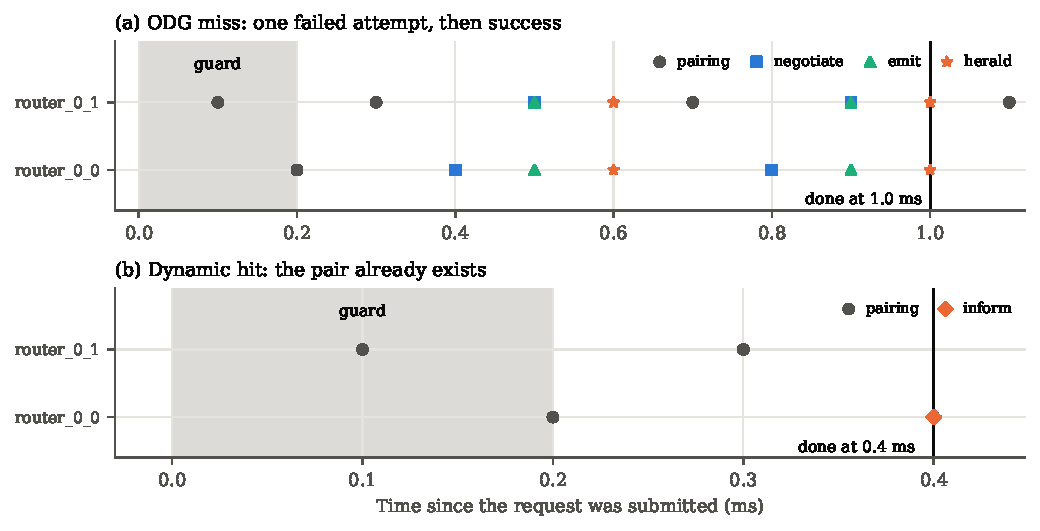
\includegraphics[width=0.96\linewidth]{timeline.pdf}
\caption{Measured events of one request on $0\to1$ (core 0 to core 1) at $\delta=100\us{}$, with time zero at submission. Markers: pairing messages, NEGOTIATE, photon emission, heralds and \code{INFORM_EP}. Source: \code{anatomy.csv}.}\label{fig:timeline}\end{figure}

\section{The formula}
Each failed attempt repeats the pairing handshake, so an attempt costs the same every time: exactly $4\delta$ ($0.4$\ms{}) on a forward hop and exactly $5\delta$ ($0.5$\ms{}) on a reverse hop, in every one of the 108 probes (minimum and maximum per-attempt time were equal). The reason is which node starts first. The extra $\delta$ appears when the node that sends NEGOTIATE (the one with the greater name) starts its protocol one message later than its partner. With $k$ attempts geometric with parameter $p$,
\[ T_{\text{gen}}=k\,c\,\delta,\quad c\in\{4,5\},\quad \mathbb{E}[T_{\text{gen}}]=\frac{c\,\delta}{p}. \]
The measured mean is \BaseGenForward{}\ms{} forward and \BaseGenReverse{}\ms{} reverse, against $0.98$ and $1.23$ predicted. The mean number of attempts is \BaseAttempts{} measured and \PredAttempts{} predicted. Figure~\ref{fig:attempts} compares the whole distribution.
\begin{figure}[htbp]\centering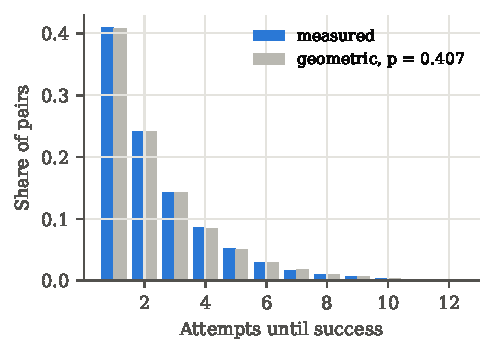
\includegraphics[width=0.5\linewidth]{attempts.pdf}\caption{Attempts until success on a forward hop, 54{,}000 pairs, against the geometric law.}\label{fig:attempts}\end{figure}

\section{What a hit costs}
A hit is not free. It costs the guard ($2\delta$) plus one or two further $\delta$: $0.4$\ms{} on a forward hop and $0.5$\ms{} on a reverse hop, with no physical attempt, whatever $p$ is. At the baseline the mean hit hop takes \QftHitCost{}\ms{}, against \QftOdgMs{}\ms{} for ODG.
\finding{Everything in a delivery is classical messaging except the photon flight. The generation time is therefore a statement about $\delta$ and $p$, and $\delta=100\us{}$ is an assumption taken from a metro-scale paper, not a chip-scale value.}

\chapter{The knobs of generation time}\label{ch:knobs}
We changed one physical knob at a time and measured single-hop generation time on both hop directions: 108 probes and \LinkPairs{} pairs in total.
\begin{figure}[htbp]\centering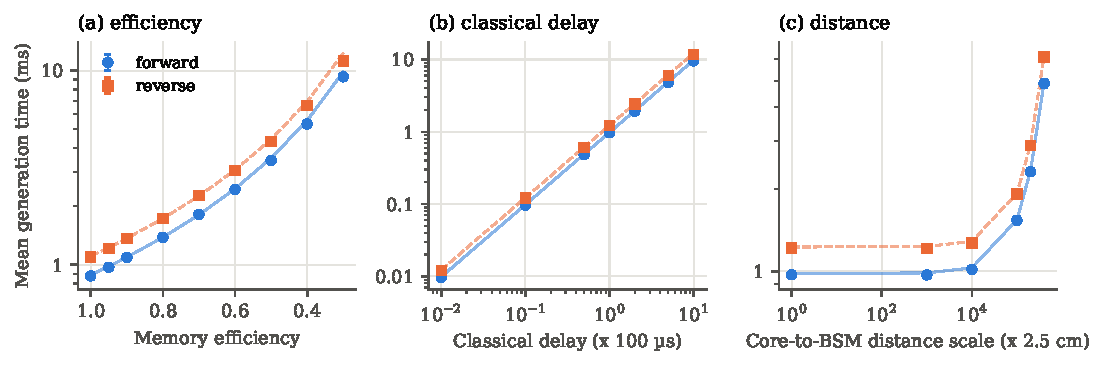
\includegraphics[width=\linewidth]{link_generation.pdf}
\caption{Mean generation time against efficiency, classical delay and distance. Points: measured, with 95\% intervals; lines: the formula. Blue: forward hop; orange: reverse hop.}\label{fig:link}\end{figure}
\begin{table}[htbp]\centering\fit{generated/link_checks.tex}
\caption{Every knob tried. ``Within tolerance'': measured mean within the interval plus 2\% of the formula's prediction.}\label{tab:link}\end{table}
\textbf{What we can say.}
\begin{itemize}
\item The number of attempts matches $1/p$ in all 108 probes, for efficiency, detector efficiency, BSM rate and fibre loss alike.
\item The time matches in 100 of 108. Four misses are efficiency 0.3 and attenuation 200\,dB/m, where about 1\% of requests exceed the 50\ms{} request window and restart; the clock then sees only the final, shorter try. That is a measurement effect, not physics. Four misses are memory excitation at 1 and 2\,kHz, where the memory itself limits each attempt (up to $+99\%$). This is a true exception to our second hypothesis. The default of 80\,MHz is far from it.
\item Distance does nothing at chip or module scale: the time is flat out to 25\,m, 5\% higher at 250\,m, and rises sharply only at kilometre scale, because both the delay and the fibre loss then grow.
\item Dark counts of $10^6$\,/s agree with the formula; $10^8$\,/s and a coherence time of $0.1$\,ms were too slow to simulate (Section~\ref{sec:limitations}).
\end{itemize}
\textbf{The equivalence of causes (H3).} Efficiency of the memory, efficiency of the detectors and the BSM success rate can each give the same $p$. We checked that the \emph{workload} result is the same whichever one is changed: 8 of 36 comparisons exceed two standard errors (1.8 expected by chance), none survives a Bonferroni correction, and the largest difference is 2.4\%. Chapter~\ref{ch:sweeps} therefore varies only memory efficiency.

\chapter{Does slower generation help Dynamic?}\label{ch:sweeps}
\section{The efficiency sweep}
Memory efficiency from 1.0 to 0.3 moves ODG generation time from 1 to 10.6\ms{}. All other settings stay at the baseline, with the 5\ms{} gap.
\begin{figure}[htbp]\centering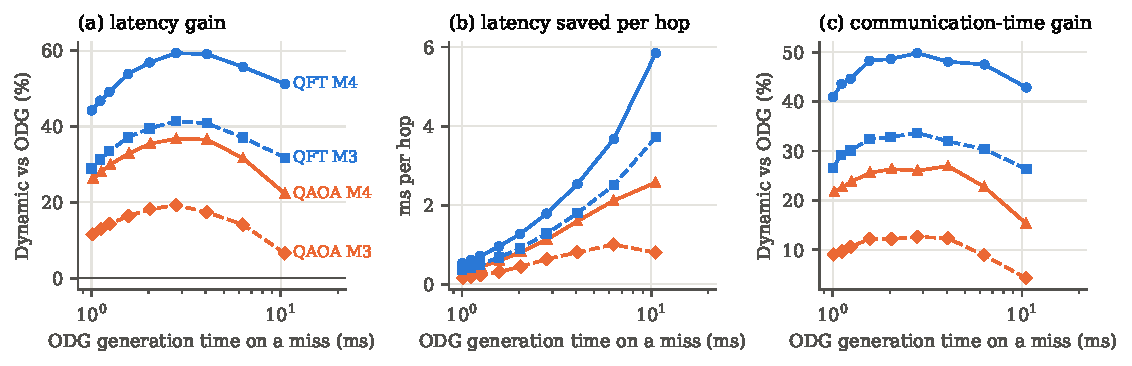
\includegraphics[width=\linewidth]{efficiency_sweep.pdf}
\caption{Dynamic against ODG on the \code{history} route as generation slows. (a) Relative latency gain; (b) absolute saving per hop; (c) gain in communication time. $M$ is memories per core; lines are labelled at the right.}\label{fig:efficiency}\end{figure}
\begin{table}[htbp]\centering\fit{generated/efficiency_sweep.tex}\caption{Efficiency sweep, \code{history}, gap 5\ms{}. Gen.\ is ODG generation time on a miss.}\label{tab:efficiency}\end{table}
\textbf{Reading the figure.} The latency gain rises, peaks at efficiency \PeakQftFourEff{} in every context, and then falls: \BaseQftFourGain{}\% $\to$ \PeakQftFourGain{}\% $\to$ \LowQftFourGain{}\% on QFT $M=4$, and \BaseQaoaFourGain{}\% $\to$ \PeakQaoaFourGain{}\% $\to$ \LowQaoaFourGain{}\% on QAOA $M=4$. Panel (b) shows why the fall is not a failure of the idea: the saving per hop grows from \BaseQftFourSaving{}\ms{} to \LowQftFourSaving{}\ms{} on QFT. The gain falls in relative terms because ODG's latency grows faster than Dynamic's once pairs stop being ready in time. The measure that falls is the \emph{share of accepted preparations that are ready}, from 100\% at the baseline to between 53\% and 68\% at efficiency 0.3.

\section{Two limits on the hit rate (H4)}
\begin{itemize}
\item \textbf{The planner's memory limit} fixes how many pairs can be prepared at all. The blocked share is the same at every efficiency (spread $0.000$ in all four contexts), and at fast generation it equals the miss rate.
\item \textbf{Preparation time against slack} decides whether a prepared pair is ready. It starts to bite only when generation takes a sizeable part of the time between launch and request.
\end{itemize}
Chapter~\ref{ch:gap} turns the second limit into a prediction.

\section{The classical-delay sweep}
Scaling the delay scales every time in a delivery equally.
\begin{figure}[htbp]\centering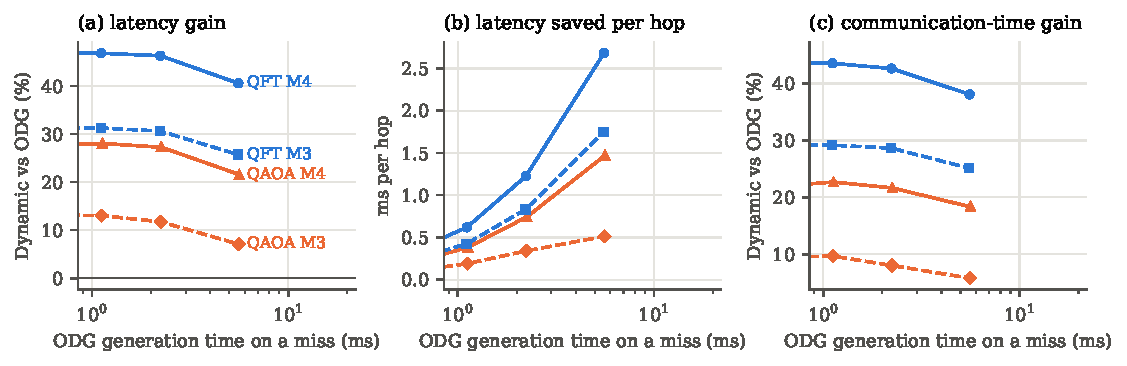
\includegraphics[width=\linewidth]{delay_sweep.pdf}
\caption{The same plot for the classical delay, $\times0.1$ to $\times5$.}\label{fig:delay}\end{figure}
For QFT the relative gain is flat from $\times0.1$ to $\times2$ (46.8\% $\to$ 46.3\%) and falls only at $\times5$ (40.6\%): the whole system scales together, and the hit rate is identical. For QAOA the gain at $\times0.1$ is lower (20\%, against 28\% at the baseline), for the reason given in Chapter~\ref{ch:time}. The absolute saving is proportional to $\delta$: $0.06$\ms{} per hop at $\delta=10\us{}$ and $2.7$\ms{} at $500\us{}$.
\finding{Slower generation helps Dynamic in absolute terms throughout, and in relative terms up to about 3\ms{} of generation time. The best case is where ODG generation takes \PeakQftFourGen{}\ms{}.}

\chapter{The hidden constant: the empty-layer gap}\label{ch:gap}
\section{What the gap is}
The compiler cuts a circuit into layers. Some layers need no inter-core request, only local gates. The simulator does not model gate time. It charges every such layer exactly 5\ms{} (\code{EMPTY_LAYER_GAP_MS}), and zero for a layer that has requests. The value has been in the code since the first import and the code comment calls it ``preserved from the legacy manager''. We found no physical reason for it. It is large: it accounts for 2.7\,s of the 3.3\,s QFT makespan. It also supplies idle time in which Dynamic can prepare pairs.

\section{The result}
\begin{figure}[htbp]\centering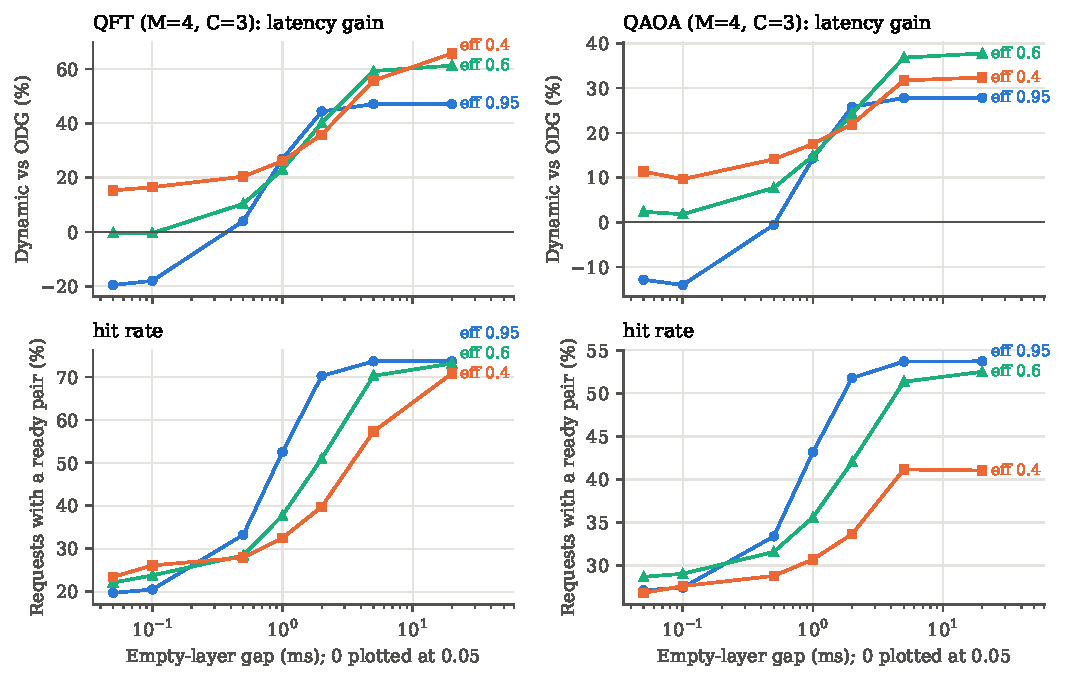
\includegraphics[width=\linewidth]{gap.pdf}
\caption{Dynamic's latency gain (top) and hit rate (bottom) against the gap, $M=4$, $C=3$, for three memory efficiencies. Zero is plotted at 0.05\ms{}.}\label{fig:gap}\end{figure}
\begin{table}[htbp]\centering\fit{generated/gap_sweep.tex}\caption{Gain in \% / hit rate in \%, for each gap, \code{history}.}\label{tab:gap}\end{table}
At the baseline efficiency and no gap, default Dynamic is worse than ODG: \QftGapZeroGain{}\% on QFT. At low efficiency and $M=4$ it still wins without the gap (QFT efficiency 0.4: $+15\%$), because ODG is then so slow that even a 20\% hit rate pays; at $M=3$ it only breaks even (QFT efficiency 0.4: $-0.5\%$). From 5\ms{} to 20\ms{} the gain does not change, so 5\ms{} already supplies enough time.

\section{Why: what happens to each planned pair}
\begin{table}[htbp]\centering\fit{generated/funnel.tex}\caption{QFT, $M=4$, $C=3$, efficiency 0.95, four seeds: what happens to the planned preparations, and what a request pays, at three gaps.}\label{tab:funnel}\end{table}
Read the table from the top. The planner promises the same 73.6 preparations per 100 requests at every gap, because it counts layers and does not know how long a layer lasts. With no gap:
\begin{enumerate}
\item Slack falls from \FunnelSlackFive{}\ms{} to \FunnelSlackZero{}\ms{}, while making a pair still takes \FunnelPrep{}\ms{} plus the guard.
\item A pair that is still being made when its request starts is not used, and the request generates its own.
\item Preparations and live requests now compete for the same four memories on each core. The protocol rejects preparations (\FunnelRejectZero{} rejection events per 100 requests, against 0), so only \FunnelAcceptedZero{}\% are accepted and \FunnelExpiredZero{}\% of pairs are made and then expire unused.
\item Requests that miss wait \FunnelMissWaitZero{}\ms{} for a free memory, against \FunnelMissWaitFive{}\ms{} with the gap and \FunnelOdgWait{}\ms{} for ODG, which never competes with preparations.
\end{enumerate}
ODG's latency does not change with the gap (1.325\ms{} in all three columns), so the extra delay comes from what Dynamic adds. The mechanism that preparations take memories from live requests is inferred from this evidence and from the rejection counts. We did not trace individual memory conflicts.

\section{A break-even model}
Let $h$ be the hit rate, $L_{\text{hit}}$ the hop latency of a hit, $L_{\text{rest}}$ the mean latency of every other request, and $L_{\text{ODG}}$ the ODG latency. Dynamic's latency is $hL_{\text{hit}}+(1-h)L_{\text{rest}}$, so Dynamic beats ODG exactly when
\[ h \;>\; h^{*} \;=\; \frac{L_{\text{rest}}-L_{\text{ODG}}}{L_{\text{rest}}-L_{\text{hit}}}. \]
This is algebra, so it fits all \BreakEvenCases{} cases by construction. What it adds is the size of the two quantities. $L_{\text{hit}}$ is almost constant, about \QftHitCost{}\ms{}. What changes is the extra cost of a non-hit over ODG, $L_{\text{rest}}-L_{\text{ODG}}$: about 0.08\ms{} with the gap, and about 0.5\ms{} without it. So the break-even hit rate rises from \QftGapFiveBreak{}\% to \QftGapZeroBreak{}\%, while the measured hit rate falls from 73.6\% to \QftGapZeroHit{}\%.
\begin{figure}[htbp]\centering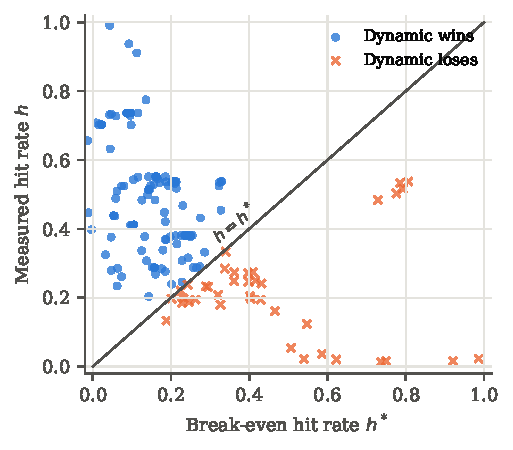
\includegraphics[width=0.55\linewidth]{breakeven.pdf}\caption{Measured hit rate against break-even hit rate in all \BreakEvenCases{} cases of the \code{history} route. Every loss lies below the diagonal.}\label{fig:breakeven}\end{figure}
\begin{table}[htbp]\centering\fit{generated/breakeven.tex}\caption{Break-even model at efficiency 0.95, $M=4$. Costs in ms.}\label{tab:breakeven}\end{table}
In the \BreakEvenLosing{} cases where Dynamic loses, the median hit rate is \BreakEvenLosingHit{}\% and the median break-even is \BreakEvenLosingBreak{}\%.

\section{Can we predict readiness?}
For an accepted preparation, the pair is ready if its attempts finish inside the slack $s$ between its launch window and its request. With $k$ geometric, $P(\text{ready}\mid s)=1-(1-p)^{\lfloor s/c\delta\rfloor}$. We read the slack distribution from each run (its 10th, 50th and 90th percentile and its maximum), so the model's only inputs are $p$, $\delta$ and the hop direction.
\begin{figure}[htbp]\centering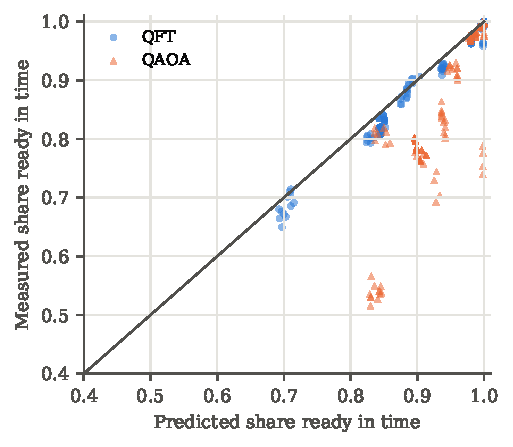
\includegraphics[width=0.52\linewidth]{readiness.pdf}\caption{Predicted against measured share of accepted preparations that were ready, in \ReadyTrials{} trials with a gap of at least 5\ms{}, lead 2 and 1\,s coherence.}\label{fig:readiness}\end{figure}
The model is accurate for QFT (mean absolute error \ReadyQftError{} points) and over-predicts QAOA at the slowest settings (mean error \ReadyQaoaError{} points, up to 30 points at efficiency 0.3). Our guess is that the percentiles we kept cannot represent QAOA's short-slack tail. We did not test that. The model is one reason we trust the ``two limits'' picture, but it is not a complete explanation for QAOA.

\chapter{Time constants and chip-scale speeds}\label{ch:time}
\section{Do only ratios matter?}
If every time constant scaled together, the latency would scale and the gain would not change. The scale test multiplies the delay, the gap, and the window sizes by 0.01, 0.1 and 2.
\begin{itemize}
\item \textbf{QFT}: the hit rate is identical at every scale (73.62\%) and the gain is 47.1\% throughout; ODG latency per unit scale is constant to better than 1\%.
\item \textbf{QAOA}: the gain moves from $+28\%$ to $-59\%$ at $\times0.01$. About 1\% of QAOA requests need a reservation retry under Dynamic (ODG has none), and each retry costs at least the fixed 1\ms{} retry wait. At $\times0.01$ the mean latency is $0.014$\ms{}, so one 1\ms{} retry per 100 requests is as large as the whole latency.
\end{itemize}
\section{The retry test}
This explanation was an inference when we first made it, so we tested it: we scaled the two retry waits together with the delay.
\begin{figure}[htbp]\centering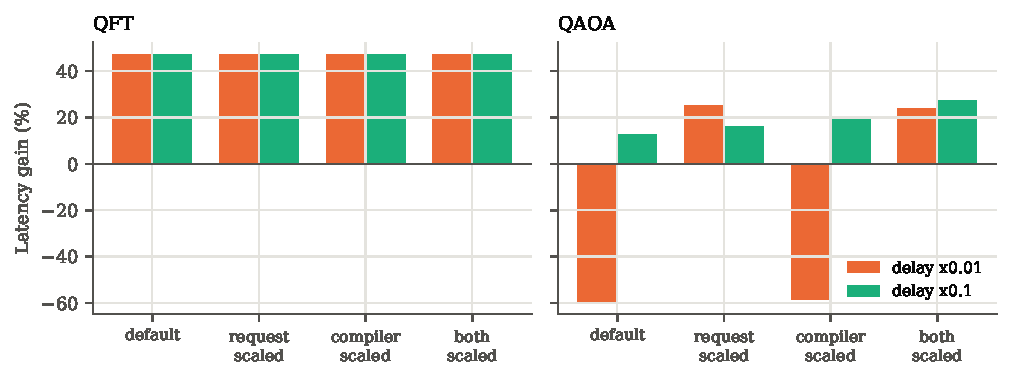
\includegraphics[width=0.95\linewidth]{retry.pdf}\caption{Latency gain at delay $\times0.01$ and $\times0.1$ when the request retry, the compiler retry, or both are scaled with the delay.}\label{fig:retry}\end{figure}
\begin{table}[htbp]\centering\fit{generated/retry.tex}\caption{Retry test, $M=4$, $C=3$, efficiency 0.95. Slowest hop shows the retry stalls.}\label{tab:retry}\end{table}
QAOA at $\times0.01$: \RetryQaoaDefault{}\% with the fixed 1\ms{} waits, and $+$\RetryQaoaScaled{}\% when both are scaled. The slowest hop falls from 1.77\ms{} to 0.11\ms{}. QFT has no retries and does not change.
\finding{At fast classical control, a 1\ms{} retry wait destroys Dynamic on QAOA. It is a fixed constant of the simulator, not a property of the strategy. Any chip-scale study of Dynamic must scale it.}

\section{Chip-scale regime}
\begin{table}[htbp]\centering\fit{generated/chip.tex}\caption{Fast control with short gaps, \code{history}, $M=4$, $C=3$.}\label{tab:chip}\end{table}
\begin{figure}[htbp]\centering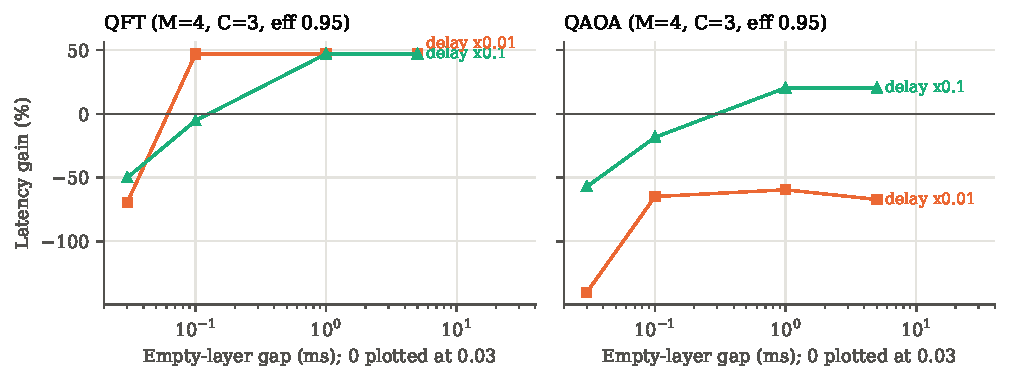
\includegraphics[width=0.95\linewidth]{chip.pdf}\caption{Latency gain against the gap at delay $\times0.01$ (1\us{}) and $\times0.1$ (10\us{}).}\label{fig:chip}\end{figure}
With the delay at $1\us{}$, QFT keeps its 47\% gain as long as the gap is at least $0.1$\ms{}, but the saving per hop is $0.006$\ms{} and the makespan gain is under 8\%: almost all of the time is the gap. QAOA stays negative at these speeds with the default retry waits (see above). The size of Dynamic's benefit therefore depends jointly on $\delta$, the gate time that a realistic gap would encode, and the retry wait.

\section{Distance}
You asked what happens with real core-to-core distances. The configured distance between cores is 5\,cm (0.025\,m from each core to the BSM halfway).
\begin{table}[htbp]\centering\fit{generated/distance.tex}\caption{Real link lengths at $M=4$, $C=3$, efficiency 0.95, four seeds.}\label{tab:distance}\end{table}
From 5\,cm to 30\,m, nothing changes beyond seed noise: light crosses 30\,m in 150\,ns, which is 670 times smaller than the $100\us{}$ added to every message. Distance would matter only at kilometre scale.

\chapter{Tuning Dynamic}\label{ch:tuning}
\section{One option at a time}
We changed one Dynamic option at a time, in 8 contexts (QFT and QAOA, $M=3$ and 4, efficiency 0.95 and 0.4), on seeds 60--63.
\begin{figure}[p]\centering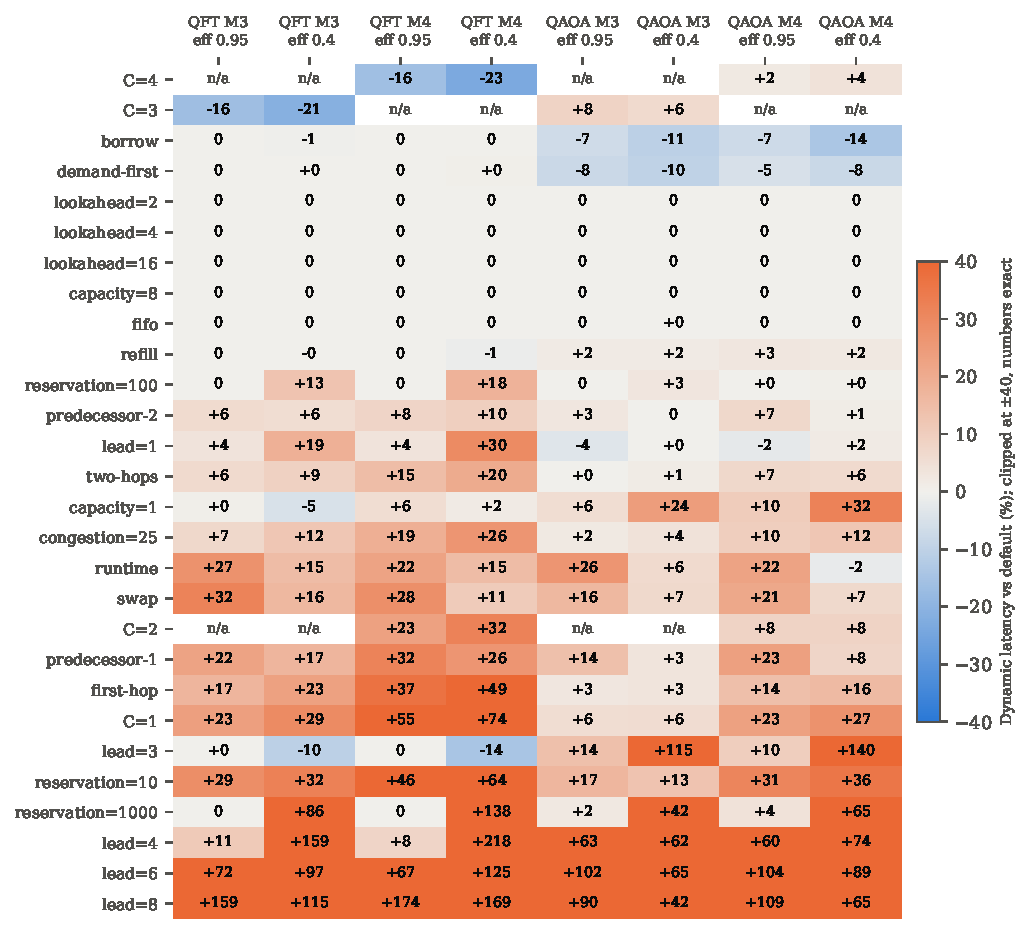
\includegraphics[width=0.84\linewidth]{tuning.pdf}
\caption{Change in Dynamic's latency against the default, in \%. Blue: better; orange: worse. The scale is clipped at $\pm40$\%; the printed numbers are exact. ``n/a'': that option is the default in that context.}\label{fig:tuning}\end{figure}
\begin{table}[htbp]\centering\fit{generated/tuning_summary.tex}\caption{Best and worst option in each context, and how many options changed latency by more than 2\%.}\label{tab:tuning}\end{table}
\textbf{What it shows.}
\begin{itemize}
\item \textbf{The default is close to a local optimum.} Of the options tried, only two families help anywhere.
\item \textbf{C=M helps QFT} by 16--23\%: letting Dynamic use the memory that was reserved for ODG-style requests. It does not help QAOA, where it is worse by 2--8\%.
\item \textbf{Borrowing pairs and demand-first help QAOA} by 5--14\%. They change nothing for QFT.
\item \textbf{Lookahead and generation capacity (8) do nothing}, which agrees with the group's earlier finding. FIFO admission is also identical.
\item \textbf{A longer lead hurts, often badly:} lead 4 made QFT 8--218\% slower and QAOA 60--74\% slower. Other options that hurt: swap, runtime planning, first-hop-only preparation, and longer reservations (+0 to +138\%).
\end{itemize}

\section{The lead depends on the speed and the gap}
\begin{figure}[htbp]\centering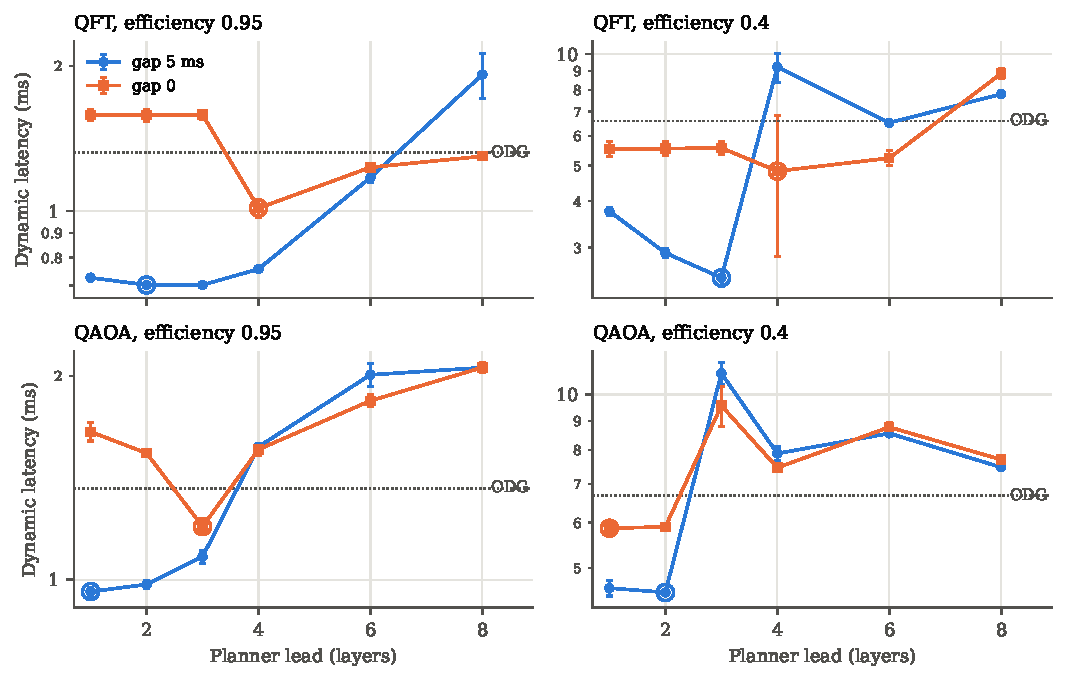
\includegraphics[width=\linewidth]{lead.pdf}\caption{Dynamic latency against the planner lead ($M=4$). Rings mark the best lead; the dotted line is ODG.}\label{fig:lead}\end{figure}
The best lead is 1, 2, 3 or 4, depending on the case: QFT at slow generation prefers lead 3 at gap 5\ms{} (2.49\ms{} against 2.90\ms{} for lead 2), and lead 4 with no gap (1.01\ms{} against 1.58\ms{} at baseline efficiency). The jump at lead 4 matches QFT's layout, which has about one active layer every four layers: the lead is counted in layers, but what matters is the time available. A planner that counts milliseconds, or active layers, would remove this tuning. Beyond lead 4, memory fills with waiting pairs and latency rises.

\section{Do the chosen options hold on unseen seeds?}
We picked, in each context, the option with the lowest mean latency if it beat the default by more than the two 95\% intervals added together, and ran it on seeds 100--105. The rule was written before the validation seeds were run.
\begin{figure}[htbp]\centering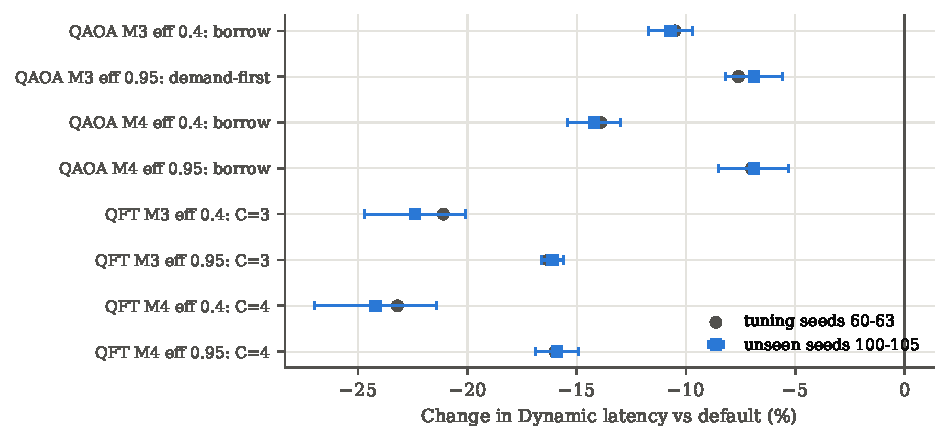
\includegraphics[width=0.85\linewidth]{validation.pdf}\caption{Latency change from the default: tuning seeds (grey) and unseen seeds (blue, with 95\% interval).}\label{fig:validation}\end{figure}
\begin{table}[htbp]\centering\fit{generated/validation.tex}\caption{Validation. ``vs ODG'' is the change in Dynamic's latency against ODG on the same seeds.}\label{tab:validation}\end{table}
All \ValidationHold{} of \ValidationTotal{} options held, with effects within about one point of tuning, and every chosen option still beats ODG. Two cautions: all seeds share one mapping per workload, and C=M removes the memory that was reserved for ODG-style requests, which matters if demand traffic can be heavier than in these workloads.

\chapter{Routes, memory, coherence and other workloads}
\section{Routes}
\begin{figure}[htbp]\centering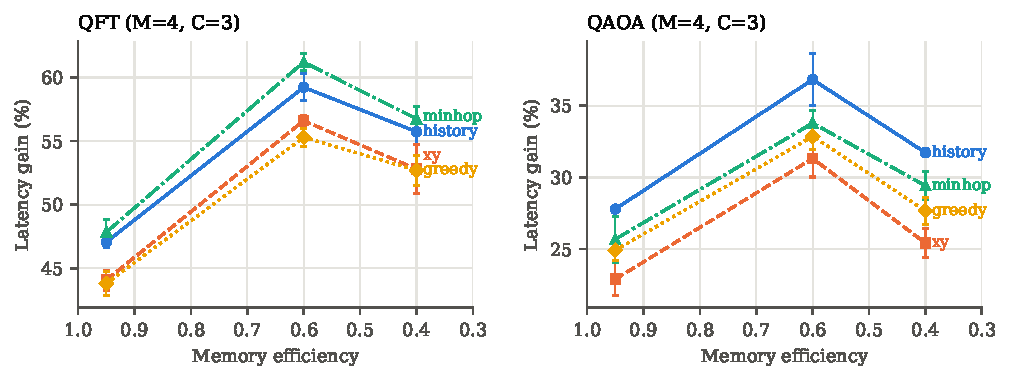
\includegraphics[width=0.95\linewidth]{routes.pdf}\caption{Latency gain by route against memory efficiency ($M=4$, four seeds, 95\% intervals).}\label{fig:routes}\end{figure}
\begin{table}[htbp]\centering\fit{generated/routes.tex}\caption{Latency gain in \% by route, $M=4$.}\label{tab:routes}\end{table}
\code{history} beats XY at every efficiency in all four contexts by 2 to 6 points (36 of 36 points of the efficiency sweep). It is best on QAOA. On QFT, \code{minhop} is slightly better (e.g. 47.8\% against 47.1\% at baseline, 61.2\% against 59.2\% at efficiency 0.6), and the differences exceed the interval. Its advantage over XY grows with slower generation only for QAOA $M=4$ (Spearman $\rho=0.82$, $p=0.007$), so our tenth hypothesis is only partly supported.

\section{Memory per core}
\begin{figure}[htbp]\centering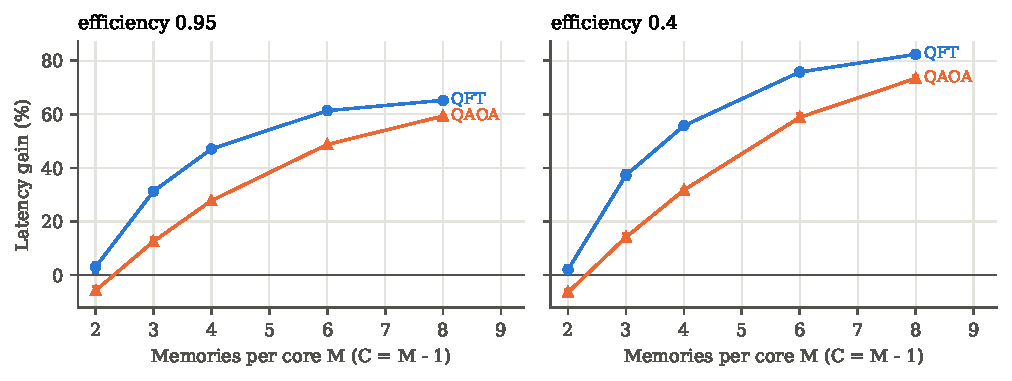
\includegraphics[width=0.95\linewidth]{memory.pdf}\caption{Latency gain against $M$ (with $C=M-1$).}\label{fig:memory}\end{figure}
\begin{table}[htbp]\centering\fit{generated/memory.tex}\caption{Memory per core. ``Planner-blocked'' is the share of requests the planner could not prepare.}\label{tab:memory}\end{table}
Memory per core is the strongest lever we found. On QFT at the baseline efficiency, the gain rises from \MemQftTwo{}\% at $M=2$ to \MemQftEight{}\% at $M=8$, because the planner-blocked share falls from 71\% to 1\%. At $M=2$, Dynamic is worse than ODG for QAOA.

\section{Coherence}
\begin{figure}[htbp]\centering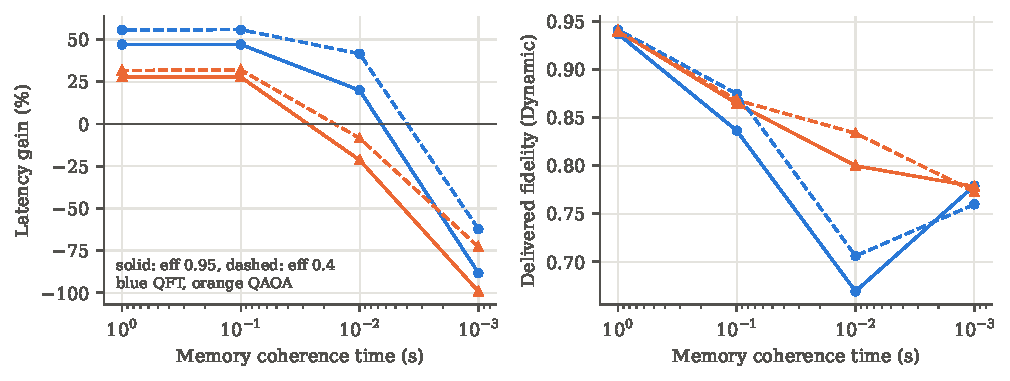
\includegraphics[width=0.95\linewidth]{coherence.pdf}\caption{Dynamic's latency gain and delivered fidelity against the memory coherence time.}\label{fig:coherence}\end{figure}
\begin{table}[htbp]\centering\fit{generated/coherence.tex}\caption{Coherence time, $M=4$, $C=3$.}\label{tab:coherence}\end{table}
Pairs wait about 9\ms{} in memory at baseline (a two-layer lead spans two 5\ms{} gaps). At coherence 100\ms{} only fidelity changes (0.94 $\to$ 0.84--0.87). At 10\ms{} pairs start to expire: the QFT gain falls from 47\% to 20\% and QAOA turns negative. At 1\ms{} Dynamic is worse than ODG by 55--99\%. The fidelity of Dynamic is not monotone at 1\ms{} (0.76--0.78) because almost no prepared pair survives, and most deliveries are then on demand. ODG's own fidelity also falls at 1\ms{}.

\section{Other workloads}
\begin{figure}[htbp]\centering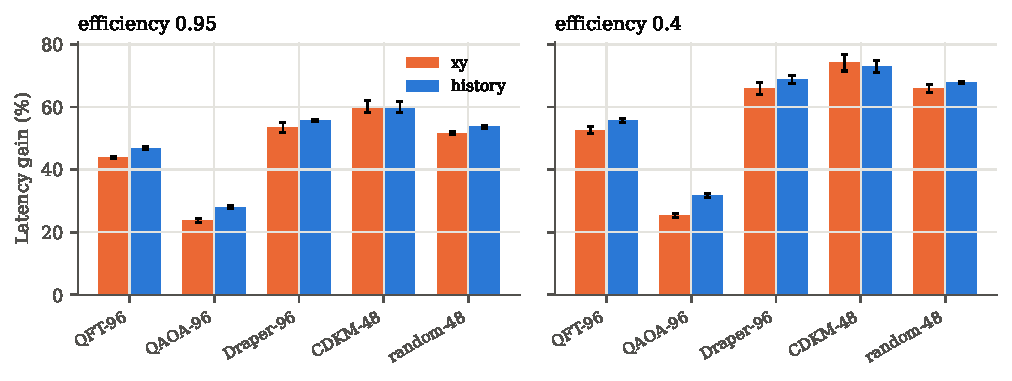
\includegraphics[width=0.95\linewidth]{workloads.pdf}\caption{Latency gain for five workloads ($M=4$, $C=3$).}\label{fig:workloads}\end{figure}
\begin{table}[htbp]\centering\fit{generated/workloads.tex}\caption{The three additional workloads, four seeds.}\label{tab:workloads}\end{table}
Dynamic wins on every workload we tried, and by more on the three additional workloads (54--60\% at the baseline). \code{history} is ahead of XY on Draper and the random circuit; on CDKM the two differ by less than their intervals.

\chapter{Hypothesis scorecard}
\begin{table}[htbp]\centering\scriptsize\begin{tabular}{@{}lp{3.2cm}p{2.6cm}p{7.0cm}@{}}
\toprule
ID & Hypothesis & Verdict & Evidence \\
\midrule
H1 & Generation time is $(4\text{ or }5)\,\delta/p$. & \textbf{Mostly supported} & Attempts: 110/110 probes inside tolerance. Time: 102/110; the 8 misses are 4 at memory excitation 1--2\,kHz (H2) and 4 where requests longer than the 50\,ms window restart (efficiency 0.3, attenuation 200\,dB/m). \\[2pt]
H2 & Only $\delta$ and the factors of $p$ matter. & \textbf{Partly falsified} & Coherence, fidelity, gap and dark counts $\le$ 1000/s change nothing (all within 14.7\%). Memory excitation below 5\,kHz does matter (+99\% at 1\,kHz). \\[2pt]
H3 & Equal $p$ gives equal results whatever its cause. & \textbf{Supported in practice} & 8 of 36 comparisons exceed two standard errors (1.8 expected by chance); none survives a Bonferroni correction; the largest difference is 2.4\%. \\[2pt]
H4 & Two separate limits on the hit rate. & \textbf{Supported} & The planner-blocked share is constant in efficiency (spread 0.000 in all four cases) and equals the miss rate at fast generation. The ready-in-time share of accepted pairs falls only below efficiency 0.6. \\[2pt]
H5 & Absolute saving grows; relative gain peaks. & \textbf{Supported} & All four contexts peak at an interior efficiency (0.6); the absolute saving grows with generation time in 3 of 4 (QAOA M3 turns at 0.4). \\[2pt]
H6 & The gap decides how much Dynamic gains. & \textbf{Supported, strongly} & With no gap, default Dynamic loses to ODG at normal speed ($-$20\% on QFT M4/C3). The hit rate responds to the gap in every context. Beyond 5\,ms the gain stops changing. \\[2pt]
H7 & Only ratios of time constants matter. & \textbf{Falsified for QAOA, then explained} & QFT: hit rate identical at every scale. QAOA at delay $\times$0.01: $-59\%$, caused by the fixed 1\,ms retry waits; scaling them restores $+24\%$ (retry test). \\[2pt]
H8 & The best lead depends on generation time. & \textbf{Supported} & Best leads found: 1, 2, 3, 4. They depend on both the gap and the generation speed, and leads above 4 are never best. \\[2pt]
H9 & Short coherence removes the gain. & \textbf{Supported} & Coherence 100\,ms changes only fidelity; 10\,ms cuts the QFT gain from 47\% to 20\% (hits fall as pairs expire); 1\,ms makes Dynamic 55--99\% worse than ODG. \\[2pt]
H10 & History's advantage grows with slower generation. & \textbf{Partly supported} & History beats XY at every efficiency in all 4 contexts, by 2--6 points. The advantage grows significantly only for QAOA M4 ($\rho=0.82$, $p=0.007$); it is flat for QFT. \\[2pt]
\bottomrule
\end{tabular}
\caption{The ten hypotheses of \code{plan.md}, each judged by the rule written before the sweeps.}\label{tab:scorecard}\end{table}

\chapter{How to think about it}
\begin{enumerate}
\item \textbf{Dynamic is ordering ahead.} A request that finds its pair ready pays only the reservation handshake and a handover: about $0.4$--$0.5$\ms{} here, whatever generation costs. ODG pays that plus generation, about $1.1$\ms{} at the baseline.
\item \textbf{A pair is useful only if it is ready in time, and only if preparing it did not delay someone else.} The first needs slack longer than generation. The second needs spare memory.
\item \textbf{Slow generation helps until it eats the slack.} Savings per hop keep growing, but past about 3\ms{} of generation time the share of pairs that are ready in time falls, and the relative gain with it.
\item \textbf{The gap is the slack.} The 5\ms{} charged per empty layer is where Dynamic gets its time. Take it away and Dynamic needs a lead counted in time, not in layers.
\item \textbf{Memory is the real limit.} At baseline speed, almost every planned pair is ready; the pairs that are missing are the ones the planner could not fit into the memories. More memory per core gains more than any tuning.
\item \textbf{Fixed constants hide in simulators.} 100\us{} per message, 5\ms{} per empty layer, and 1\ms{} per retry together decide the absolute numbers, and two of them decided a sign in this study.
\end{enumerate}

\chapter{Recommendations}
\begin{enumerate}
\item \textbf{State results as ratios and regimes.} The absolute latencies depend on constants that are not hardware values. Quote the gain, the hit rate and the break-even, and say which constants were used.
\item \textbf{Ask the supervisor for the target platform}, then fix the three constants together: the classical delay, a gap built from gate times, and the retry waits. Our results give the sensitivity for each.
\item \textbf{For the default configuration}, keep lead 2 (lead 3 for slow generation), and use C=M for QFT-like circuits and borrowing or demand-first for QAOA-like circuits. All three held on unseen seeds.
\item \textbf{Change the planner to count time.} The best lead differs across contexts because the planner counts layers. A slack in milliseconds would remove the tuning and the collapse at no gap. This is the most promising code change we see.
\item \textbf{Add more memory per core before tuning anything else.} Moving from $M=4$ to $M=6$ is worth more than every option we tried.
\item \textbf{Next experiments:} a planner that counts time; gate times for the gap; more than one mapping per workload; a fidelity threshold; torus topology; and data teleportation timing.
\end{enumerate}

\chapter{Limitations and threats to validity}\label{ch:limits}
\begin{itemize}
\item \textbf{One mapping per workload.} Seeds vary the simulator's randomness only. Intervals therefore understate the uncertainty about other circuits or mappings. Five workloads help, but they are five mappings.
\item \textbf{Assumed constants.} The delay, the gap and the retry waits are not calibrated to hardware.
\item \textbf{Reduced matrix.} Seeds are 4 to 10 per setting, and some grids are coarse. Gains are quoted with their intervals.
\item \textbf{Inferences, not tests.} The statement that preparations take memory from live requests comes from the funnel and the unchanged ODG latency, not from tracing conflicts. The reason the readiness model over-predicts QAOA was not tested.
\item \textbf{Single-link gaps.} Dark counts of $10^8$\,/s and coherence 0.1\,ms could not be simulated in a practical time (Section~\ref{sec:limitations}).
\item \textbf{Fidelity.} No pair is rejected for low fidelity, so a Dynamic pair that waits 9\ms{} still counts. The reported delivered fidelity is a mean over pairs, not a circuit success probability.
\end{itemize}
\section{The single-link settings that were hard to simulate}\label{sec:limitations}
Dark counts of $10^6$ and $10^8$ per second and a coherence time of $0.1$\,ms did not finish 3000 samples in the first screen (15 minutes each), because they create events every microsecond or faster. They were rerun with a time limit:\par\smallskip
\begin{center}\small\begin{tabular}{llrrr}
\toprule
Setting & Hop & Outcome & Generation (ms) & Fidelity \\
\midrule
dark counts $10^6$\,/s & 0$\to$1 & 100 samples & 1.116 & 0.950 \\
dark counts $10^6$\,/s & 1$\to$0 & 100 samples & 1.200 & 0.950 \\
dark counts $10^8$\,/s & 0$\to$1 & did not finish in the time limit & -- & -- \\
dark counts $10^8$\,/s & 1$\to$0 & did not finish in the time limit & -- & -- \\
coherence $0.1$\,ms & 0$\to$1 & did not finish in the time limit & -- & -- \\
coherence $0.1$\,ms & 1$\to$0 & did not finish in the time limit & -- & -- \\
\bottomrule
\end{tabular}
\end{center}
Dark counts of $10^6$\,/s (100 samples per hop) agree with the formula within the interval and leave fidelity unchanged, so the rule that dark counts do not matter holds up to $10^6$\,/s. The other two settings, run with 30 samples and a 7-minute limit, still did not finish: they are too expensive to simulate, so we say nothing about them. A setting that did not finish is part of no conclusion.


\appendix
\chapter{Reproducing the study}
All commands run from the repository root with the pinned SeQUeNCe engine on \code{PYTHONPATH} (or \code{SEQUENCE_ENGINE}).
\begin{small}\begin{verbatim}
python tools/generation_time_study/build_traces.py            # routes the frozen mappings, checks XY/greedy
python tools/generation_time_study/link_sweep.py              # single-link screening
python tools/generation_time_study/anatomy.py --output <data>/anatomy.csv
for e in efficiency delay gap lead_gap tuning memory coherence \
         routes workloads chip scale equivalence distance retry; do
    python tools/generation_time_study/run_matrix.py $e --workers 8; done
python tools/generation_time_study/collect.py                 # data/*.csv
python tools/generation_time_study/choose_tuned.py            # data/tuned_choices.json (tuning seeds only)
python tools/generation_time_study/run_matrix.py validation   # unseen seeds
python tools/generation_time_study/audit_runs.py              # every case checked against its spec
# then: hypotheses.py, model.py, model_breakeven.py, validate_choices.py
# then: figures.py, make_tables.py
cd docs/latex/generation_time_study/report && tectonic main.tex
\end{verbatim}\end{small}
\chapter{File map}
\begin{small}\begin{tabular}{@{}p{6.4cm}p{9.2cm}@{}}\toprule
Path (data files are under \path{docs/research/generation-time-2026-11-01/}) & Contents \\\midrule
\path{tools/generation_time_study/} & the code: knobs, runner, experiments, collection, tests (14 pass) \\
\path{docs/research/generation-time-2026-11-01/plan.md} & hypotheses, falsification rules, deviations \\
\path{data/*_summary.csv} & mean, spread and 95\% interval per setting \\
\path{data/*_trials.csv.gz} & one row per strategy and seed, \TotalTrials{} in all \\
\path{data/link_screen.csv}, \path{data/anatomy.csv} & single-link probes, message-level timeline \\
\path{data/hypotheses.json}, \path{data/model_*.csv}, \path{data/validation_check.csv}, \path{data/audit_runs.json} & the analyses \\
\path{results/generation_time_2026-11-01/traces/} & the 14 routed traces used \\
\path{docs/latex/generation_time_study/report/} & this report, its figures and generated tables \\\bottomrule
\end{tabular}\end{small}
\chapter{Provenance}
\begin{small}\begin{tabular}{@{}ll@{}}\toprule
Study branch & \code{abisfa/epr-generation-time-study} \\
Simulator commit studied & \code{dfd4b839} (main at the start of the study); rechecked on \code{e4db6bfa} \\
Engine & SeQUeNCe 0.8.1, commit \code{cf5283cd} \\
Python / libraries & 3.13; numpy, scipy, pandas, matplotlib \\
Report built with & tectonic \\
\bottomrule\end{tabular}\end{small}

\end{document}
